\chapter{Related Work}
\label{chap:related}

\section{Program Analysis Tools}
Program analysis tools are designed to aid developers when developing software by automating the writing, analysis, and modification of source code.
Often, program analysis is discussed as synonymous with static analysis~\cite{nielson2015principles}. 
For the purpose of my research, I define a program analysis tool as \emph{a recommendation system that performs program analysis, whether it be static or dynamic analysis, and provides information to develoeprss regarding the source code being analyzed}~\cite{robillard2014recommendation}.
Examples of program analysis tools include, but are not limited to, static code analyzers, code coverage tools, code smell detectors, and refactoring tools~\cite{adolph2011using,Murphy-Hill:2010:Ambient,ge2012reconciling}.
Program analysis tools can be used in integrated development environments (IDEs) as well in most text editors that can be used for programming, such as Vim~\footnote{http://www.vim.org/} or Emacs~\footnote{https://www.gnu.org/software/emacs/}. 
In the following sections, I will define and discuss static analysis and dynamic analysis tools separately; the reader should note that although I discuss static and dynamic analysis separately, it is not uncommon to find program analysis tools that combine static and dynamic analysis~\cite{ernst2003static}.                                                

\subsection{Static Analysis Tools}

Static analysis tools are designed to aide developers when developing software by statically analyzing source code, pre-runtime, and providing the developer with feedback about the state of their code~\cite{ernst2003static}.
Typically, static analysis works by examining the current state of the program, predicting how the program may react in that state at runtime, and reporting any information they deem necessary to the developer. Static analyses are often more conservative than dynamic analyses; this is to reduce the potential for false positives, as in most cases static analysis cannot say with 100\% certainty what will happen during run-time~\cite{ernst2003static}. 
Examples of static analysis tools include defect detectors, such as FindBugs, compilers, code smell detectors, and refactoring tools.
% TODO talk about what static analysis can do/find to motivate further

Let's use the example of FindBugs,\footnote{http://findbugs.sourceforge.net/factSheet.html} an open source static analysis tool, to better understand how static analysis tools work. FindBugs statically analyzes code to report potential defects. FindBugs determines the potential for defects using \emph{bug patterns}. Bug patterns are code idioms that map to errors, found in Java \emph{bytecode}. Bytecode, in Java, represents the compiled Java class files. Because FindBugs analyzes code without executing it, there is a heightened risk for \emph{false positives}. False positives are defects detected that will never manifest during run-time. When FindBugs finds a potential defect, it alerts the developer using notifications that provide information regarding the defect. I will discuss tool notifications in more detail in Section~\ref{subsec:comm}.


\subsection{Dynamic Analysis Tools}

Dynamic analysis tools are designed to aide developers when developing software by analyzing source code during run-time and providing the developer with feedback about runtime behavior~\cite{ernst2003static}.
Dynamic analysis works by executing the program and then making observations about program execution; because dynamic analysis runs the code, it is typically more precise than static analysis. Though dynamic analysis can produce more precise results in a similar amount of time as static analysis, dynamic analysis execution is less likely to generalize to future executions since it is based on a set of inputs that can, and probably will, change for each execution.
Examples of dynamic analysis tools include testing, code coverage, and profiling tools.

Let's use the example of Cobertura,\footnote{http://cobertura.github.io/cobertura/} an open source dynamic code coverage tool, to better understand how dynamic analysis tools work. Cobertura executes source code using JUnit test cases and reports to the user what parts of the code got covered during execution and what parts did not. Because Cobertura executes the source code, it can communicate precisely regarding the flow of the program during run-time. A static code coverage tool could speculate how much of a code base would be covered based on test cases, and possibly even a set of inputs; however, it would require more effort and be more likely to produce false positives than a dynamic code coverage tool. On the down side, the test suites a developer writes may not be characteristic of all possible executions of the program, thereby lowering the generalizability of dynamic analyses.

\begin{figure} [ht]
	\centering
	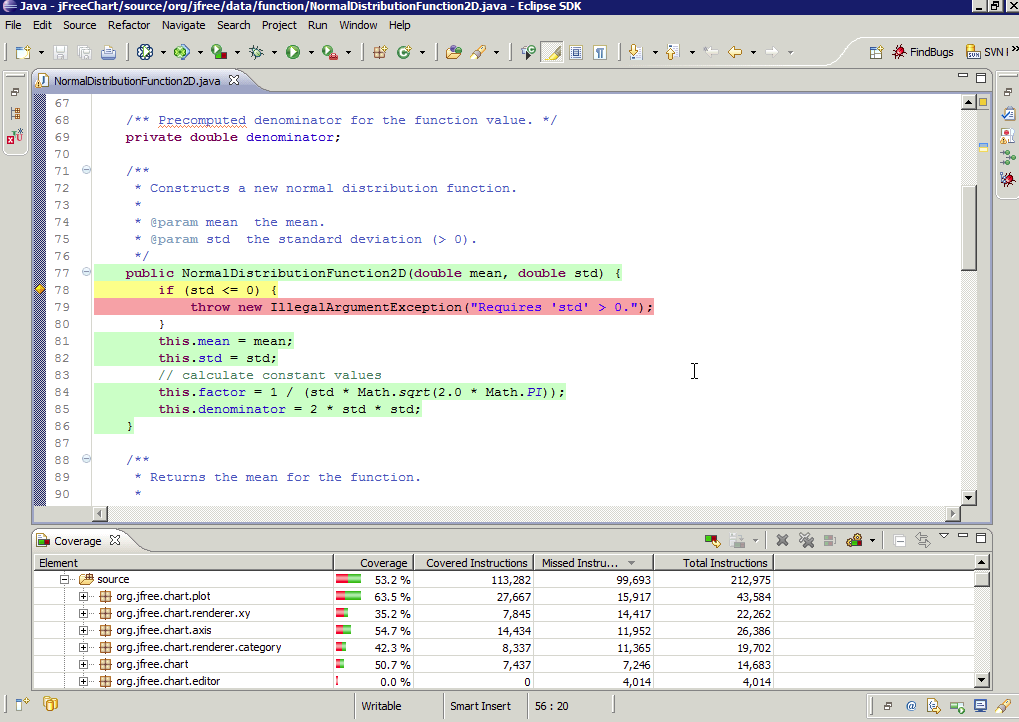
\includegraphics[width=\textwidth]{Chapter-2/figs/eclemma.png}
	\caption{EclEmma notifications in the Eclipse IDE.}
	\label{fig:ecl}
\end{figure}


\subsection{Communication via Notifications}\label{subsec:comm}

One common thread between program analysis tools like FindBugs and Cobertura is that they use \emph{notifications} to communicate with the developer. Figure~\ref{fig:eclipse} and Figure~\ref{fig:ecl} provide examples of tool notifications. 
A notification, when speaking in terms of program analysis tools, is typically a combination of visuals and text used to communicate a message to its user; for program analysis tools, the user is the developer.
Text editors like Vim and Emacs rarely include any visual components, however, because text editors are a simpler versions of IDEs, research on notifications in IDEs are more likely to also apply to text editors than vice versa. 
Therefore, I focus my research on notifications inside IDEs.

Notifications across tools vary; some provide lots of text (like FindBugs) with few visual aides, some use primarily visual means of communications (like Cobertura). Notifications can also have different goals, which may influence how developers design notifications. For example, the goal of a notification from Coverity~\footnote{http://www.coverity.com/}, another static analysis tool, is to explain a potential defect in the developer's source code and, ideally, help the developer make a decision about the defect (i.e. whether and how to resolve). Because Coverity's goal is to explain, we expect to see textual notifications that provide that explanation.
The goal of code coverage notifications is to statically show dynamic program behavior and help the developer determine the effectiveness of her test suite. EclEmma, another code coverage tool, uses colors applied directly to the source code to communicate as opposed to text. Though EclEmma also uses text to communicate code coverage (i.e. \texttt{1 of 2 branches missed} on a partially covered \texttt{if} statement), this does not allow the developer to scan the program for areas in most need of attention. Therefore, EclEmma uses other visuals, such as the bar visuals in the Coverage View (Figure~\ref{fig:ecl}) to show coverage on a given package or class.
 % TODO talk about how different parts of notification communicate for each tool; make sure it ties back to goals (defects and test coverage)!

The list of tools and notifications tools use can go on and on, but for the purposes of my research, the general definition I will use for a notification is \emph{a combination of visual and textual interfaces used by a program analysis tool to communicate information to developers about their source code.} Notifications can vary regarding what information and how much detail they provide, however, there are commonalities across tool notifications that informed this definition, which I will discuss next.

\subsection{Typical Notification Components}
% based on robilliard book
One reason I talk about program analysis tools as a type of recommendation system is because they provide information to developers completing software engineering tasks~\cite{robillard2014recommendation}. 
Another reason is that program analysis tools use the same strategies defined by Robillard as typical of recommendation systems: 1) strategies for getting the user's attention and 2) descriptive interfaces.
Program analysis tools use these strategies when communicating with developers via notifications.

There are a variety of ways that a tool can get the attention of its user~\cite{robillard2014recommendation}. Program analysis tool notifications get the attention of developers in their IDEs in one or more of the following ways: icons, dashboards, pop-ups, affordance overlays, annotations, or email notifications.
Once the tool has the developer's attention, program analysis tool notifications provide descriptive interfaces that convey information about a developer's source code. 
Information is conveyed using some combination of textual, visual, and sometimes transformative descriptions.

Some tools, like FindBugs and most IDE compilers, use icons to get developers' attention. Using the same icons, developers can access more information either by hovering over or clicking the icon. Although the icons are visual, most of the description provided by these tools is textual. As stated previously, these kinds of notifications are most common with static analysis tools as they typically need to be more descriptive. However, dynamic analysis tools like Veracode~\footnote{http://www.veracode.com/products/dynamic-analysis-dast/dynamic-analysis}, which communicate about defects similar to the ones reported by FindBugs and Coverity, also use icons and text descriptions to pass along information to the developer.

\begin{figure}
	\centering
	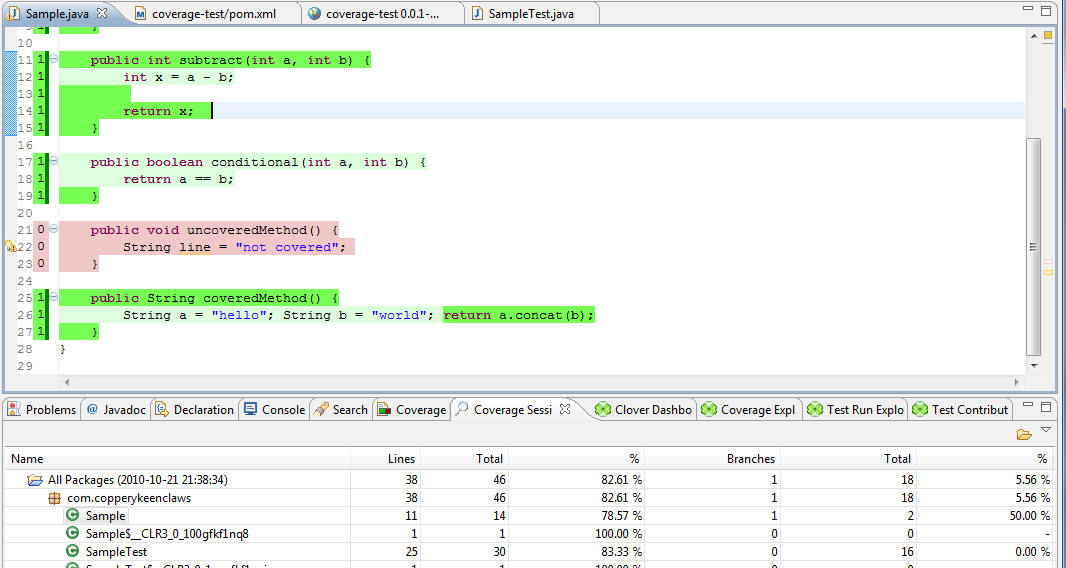
\includegraphics[width=3in]{Chapter-2/figs/cobertura.png}
	\caption{Notifications provided by Cobertura regarding code coverage.}
	\label{fig:cobertura}
\end{figure}

\begin{figure}
	\centering
	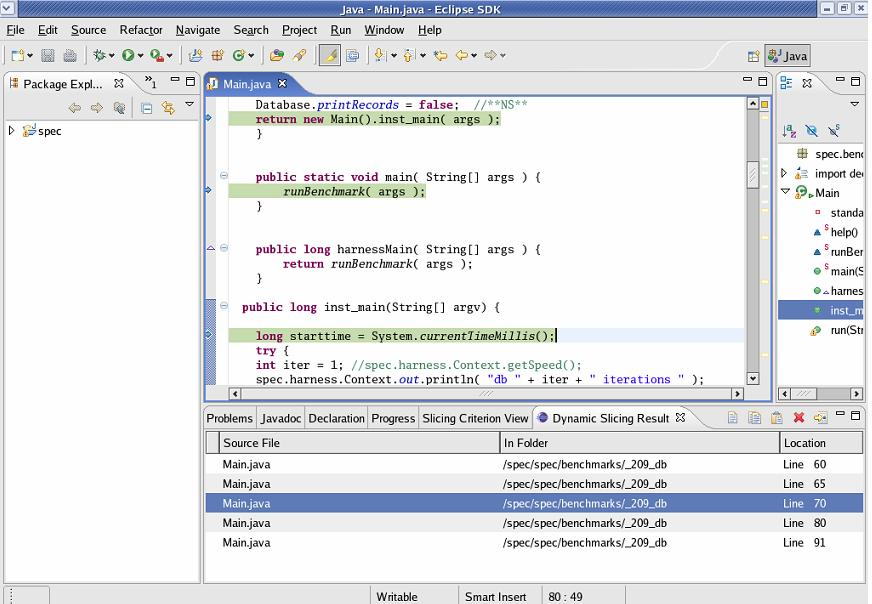
\includegraphics[width=3in]{Chapter-2/figs/jslice.jpg}
	\caption{Notifications provided by JSlice regarding a dynamic slice of the program.}
	\label{fig:jslice}
\end{figure}


Some tools use affordance overlays or annotations to both get the attention of the developer and for the descriptive interface. For example, Cobertura and JSlice~\footnote{http://jslice.sourceforge.net/} use affordance overlays in the form of source code highlighting, as shown in Figure~\ref{fig:cobertura} and Figure~\ref{fig:jslice}, to alert the developer of and communicate about dynamic behavior. Coverity Dynamic Analyzer~\footnote{http://www.coverity.com/library/pdf/Coverity-Dynamic-Analysis.pdf}, which is similar to Veracode, uses annotations, such as the one in Figure~\ref{fig:coverity} in the editor to communicate about defects in the code.

\begin{figure}
	\centering
	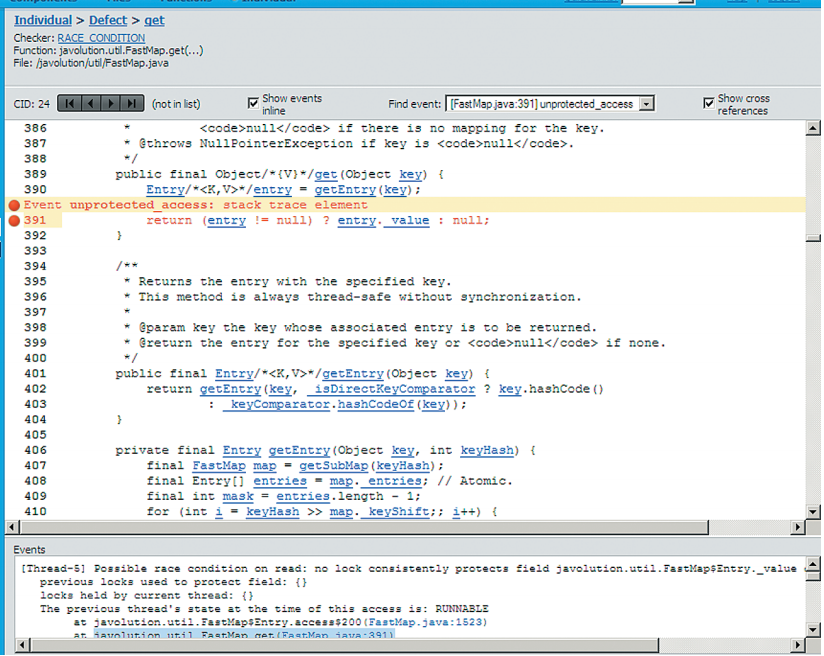
\includegraphics[width=3in]{Chapter-2/figs/coverity-dynamic.png}
	\caption{A notification provided by Coverity regarding a race condition.}
	\label{fig:coverity}
\end{figure}

A small subset of tools use dashboards, such as the one shown to the right in Figure~\ref{fig:stench}. StenchBlossom, a code smell detection tool gets and maintains a developer's attention using an ambient dashboard~\cite{Murphy-Hill:2010:Ambient}. At anytime the developer is interested in the information being provided by the tool, the developer can use options in the dashboard to explore code smells present in their code base. The description is visual, using color overlays that map to each type of code smell. 

\begin{figure}
	\centering
	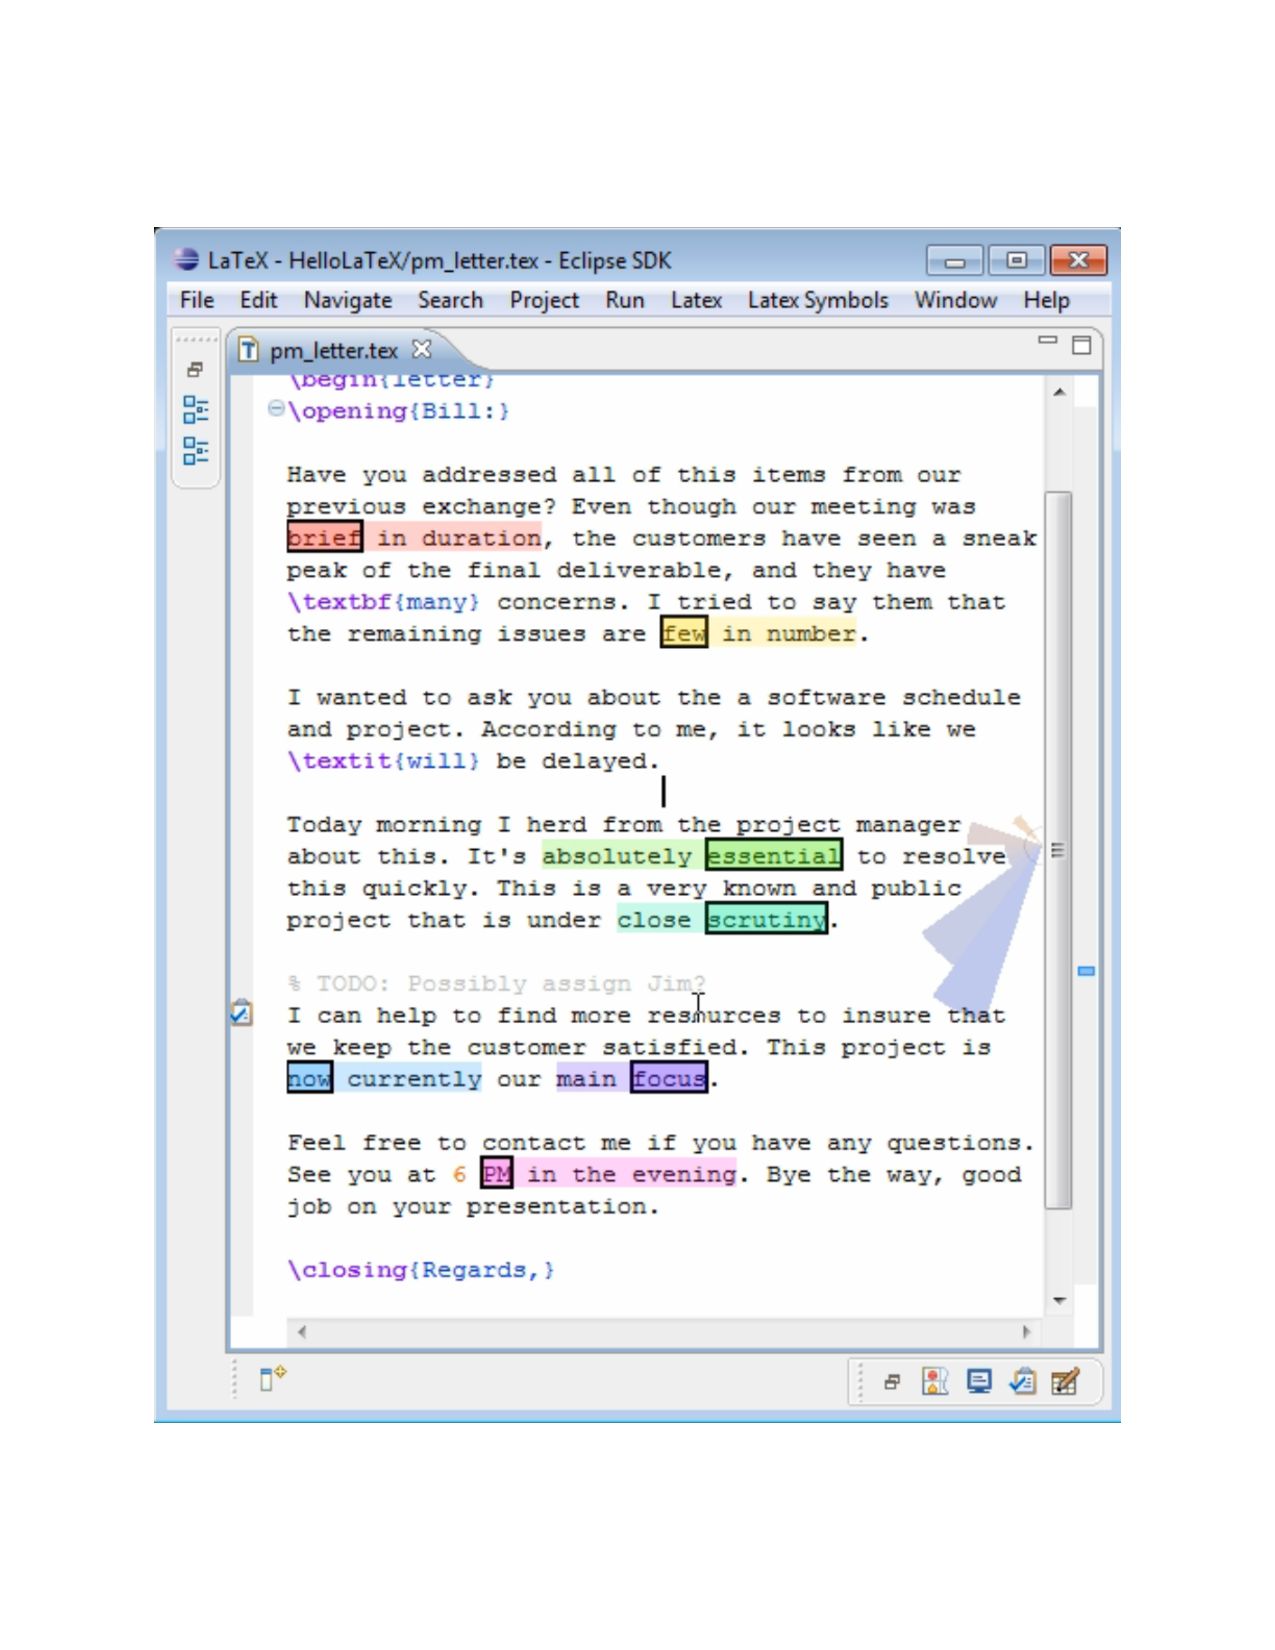
\includegraphics[width=3in]{Chapter-2/figs/stenchblossom.pdf}
	\caption{Notifications provided by StenchBlossom regarding code smells.}
	\label{fig:stench}
\end{figure}

\begin{figure}
	\centering
	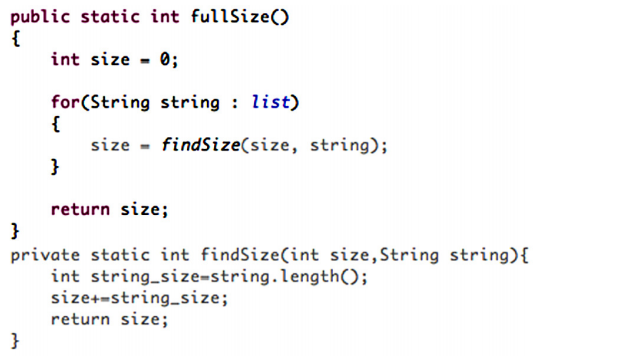
\includegraphics[width=3in]{Chapter-2/figs/witchdoctor.png}
	\caption{A notification provided by WitchDoctor regarding a refactoring that's taking place.}
	\label{fig:witch}
\end{figure}

Finally, an even smaller subset of program analysis tools provide transformative descriptive interfaces. Transformative interfaces provide the developer with some idea of how the suggestion being made would affect the task at hand. For example, WitchDoctor, a refactoring tool, detects refactorings and then makes the developer aware of their refactoring by offering to complete the refactoring for the developer. To inform this process, WitchDoctor provides information regarding the assumed refactoring by showing the developer within their text editor what will happen if the refactoring is applied, as shown in Figure~\ref{fig:witch}.


% types of descriptions (text and visual)
% goals of information provided (??)

\subsection{Breaking Down the Code Developers Write \& Tools Analyze}

% communicate about the state of with source code
The goal of program analysis tool notifications is to communicate some information to the developer about her source code about the task at hand.
The source code a developer writes is a runnable manifestation of programming-oriented and human-oriented concepts~\cite{van2004concepts,biggerstaff1994program}. 
At the lowest, most fundamental level, are \emph{programming-oriented concepts}, which relate to how the source code maps to programming language concepts. For simplicity, I will refer to these concepts simply as programming concepts.
Programming concepts can be as simple as the means for storing and passing data, such as variables, or as complex as the means for structuring data, such as generics~\cite{jazayeri1997programming}.
At a more abstract level, \emph{human-oriented concepts} relate to the high level requirement of the source code, such as ``acquire target'' or ``complete transaction''.

Typically a given notification is associated with only one human-oriented concept, though not all tools communicate about human-oriented concepts. For example, refactoring tools do not communicate about requirements such as ``acquire target.'' These kinds of tools typically focus on programming concepts; refactoring tools attempt to communicate about programming concepts such as variables and modules.
On the flip side, there can be more than one notification pertaining to a one human-oriented concept and one notification can communicate about more than one programming concept. 

\begin{figure} [ht]
	\centering
	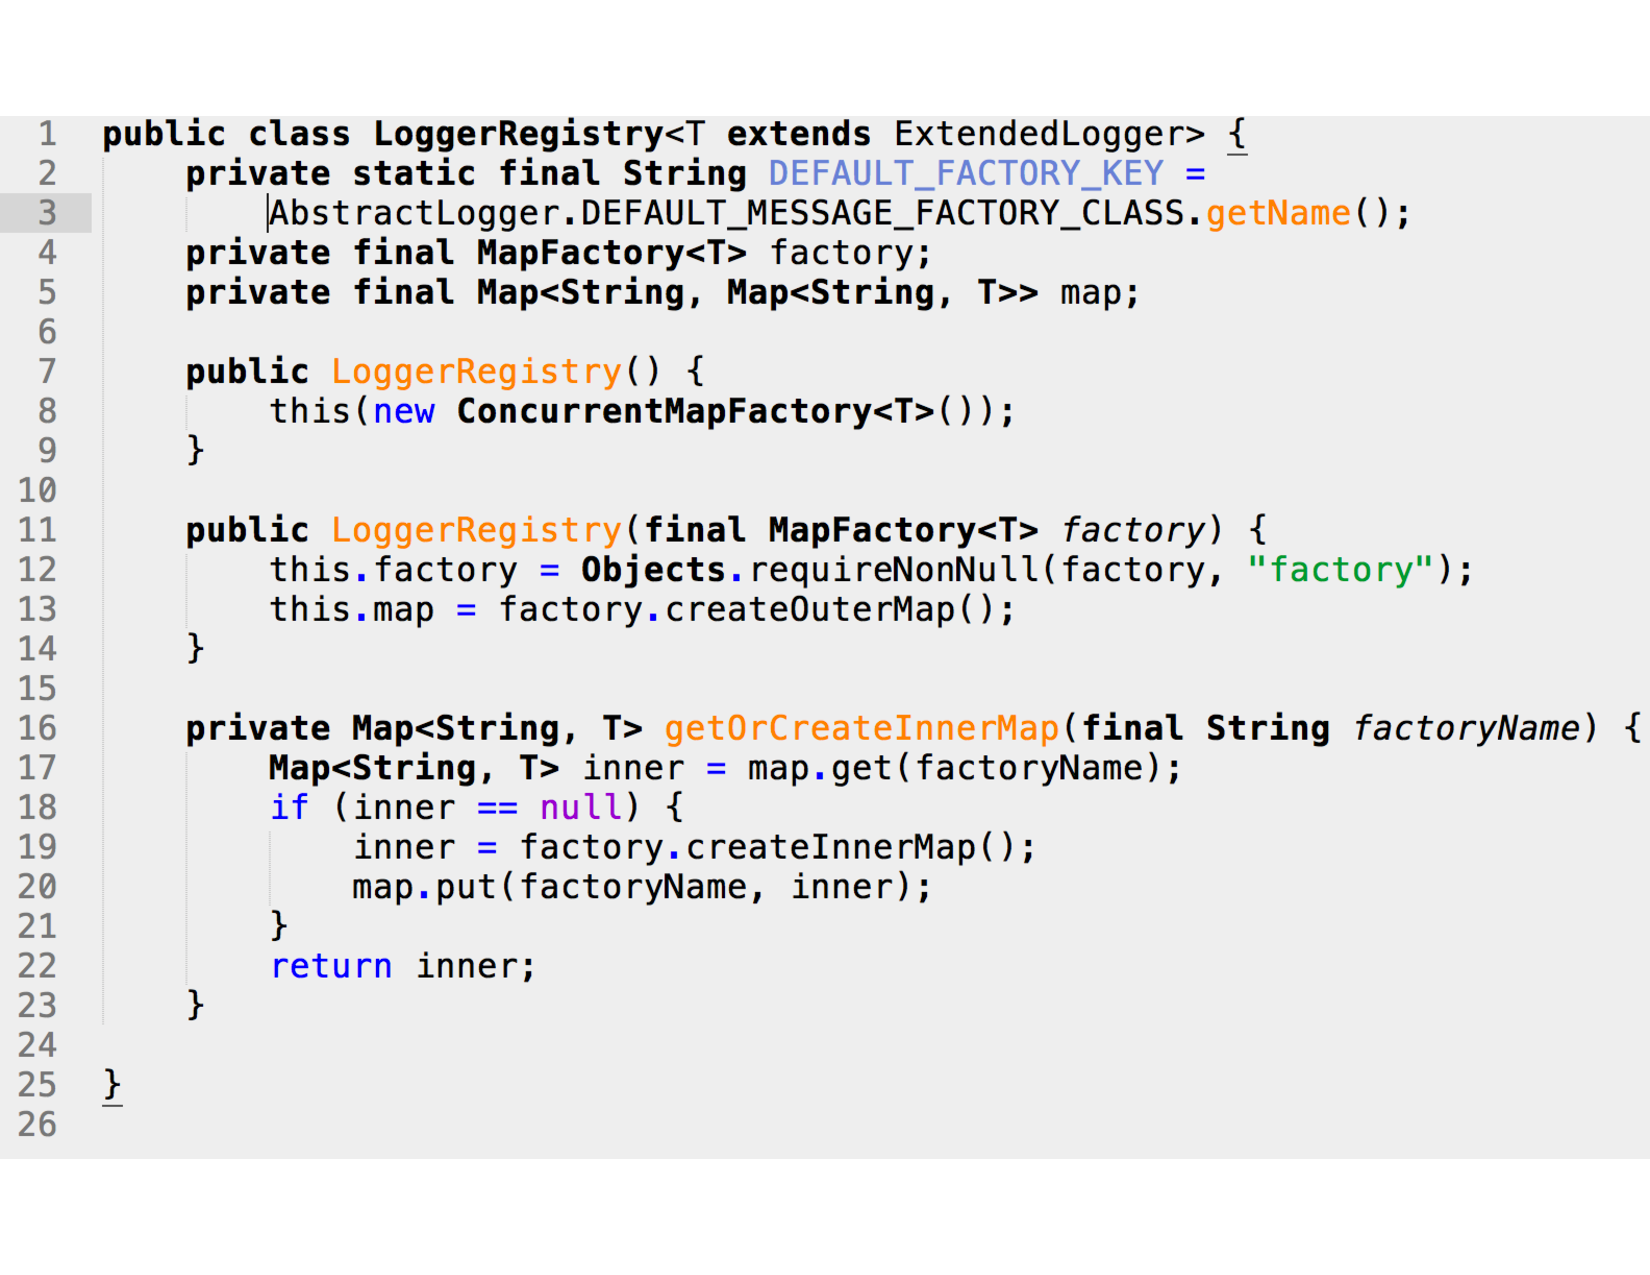
\includegraphics[width=\textwidth]{Chapter-2/figs/code-example.pdf}
	\caption{A source code example for writing to a log file.}
	\label{fig:code}
\end{figure}

Consider, for example, the following source code in Figure~\ref{fig:code}. The requirement, or human-oriented concept, at play is ``write to log file''. If a notification was attached to this code, it would be telling the developer something about the code she wrote to ``write to log file''.
There are multiple programming concepts at play, which aligns with the types of notifications the developer could get. 
In the process of writing this code, the developer could get a notification regarding any number of programming concepts (buffered streams, exception handling); for example, tools like FindBugs, Sonar, and IntelliJ's built-in static analyzers notify developers when they have opened a stream (\texttt{BufferedWriter} in the above example) and there is a possibility the stream that is writing to the file is not closed.
A developer may also get a notification regarding exception handling. Here, the developer has written code to catch an \texttt{IOException} if it occurs. However, if she did not implement code to deal with the potential for an \texttt{IOException} she would get a compiler notification communicating the need to do so.


% TODO later, should note that focusing on programming oriented concepts because those generalize and are foundational to developing the abstractions that are human oriented concepts (biggerstaff)


% RELATED WORK

Research related to mine falls under the following categories: evaluating and improving tool usability, improving notification understanding and resolution, predictive user models, and developer knowledge representation.

\section{Program Analysis Tool Usability}
% TODO: make sure exhaustive here; check studies on dynamic analysis tools too!

There have been many studies on program analysis tools, many of which focus on
their correctness and functionality~\cite{Ayewah:2008:FindBugs,Bessey:2010:Coverity,dugan2000developing,luk2005pin}.
Unlike existing work, which typically focuses on one type of program analysis tool, my work focuses on developers' perception on 
using different types of program analysis tools, what may have caused their perceptions, and how we can build on or improve their perceptions. 
Perception plays an important role in when considering human and computer interactions~\cite{Dastani:2002:Perception} and
can be influenced by a number of things, such as the subjective preferences of
the user.

% TODO: flesh this out
Pettit and colleagues studied the effect of enhanced compiler messages for students\cite{pettit2017enhanced}.
They found no significant improvement, based on likelihood of successive compiler errors, compiler error occurrence, and progress students make towards successful project completion.
Their enhancements were designed without rationale, only focusing on students. Also, the information the was same no matter how much students already knew. Enhancements were made based somewhat on assumed knowledge; the adaptations I am proposing would be based on actual knowledge.
I also assessed other types of enhancements, such as inclusion of examples and links to external information.

Hamou-Lhadj and Lethbridge surveyed trace exploration tools to determine how these tools 
can be used by developers and potential improvements to trace exporation tools~\cite{hamou2004survey}. 
Based on their evaluation of the tools, they found that areas 
for improvement for these type of tools include visibility during trace removal and automated suggestions.
Pacione and colleagues conducted a case study on five dynamic visualization tools that perform either static or dynamic code analysis and observed the output provided~\cite{pacione2003comparative}. Pertaining to usability, they found that level of abstraction can make a difference when explaining large scale problems.

Storey and colleagues ran user experiments with 12 developers on two approaches for presenting software structure in a reverse engineering system~\cite{storey1997rigi}. They found that certain interfaces are better for low-level tasks and that users prefer reverse engineering tools with consolidated interfaces, rather than multiple windows.
Bennett and colleagues conducted interviews and user experiments to evaluate the usability and potential improvements of their sequence diagram creation and exploration tool~\cite{bennett2008survey}. Sequence diagram tools create sequence diagrams using static analysis, dynamic analysis, or both.
Much of the feedback developers provided suggested search and selection highlighting are both useful feature for sequence diagram tools, though there are improvements that can be made to existing implementations.


Ayewah and Pugh conducted a study where they claimed that static analysis tools
should help engineers find bugs as early as possible in the development cycle,
when they are cheap to fix~\cite{Ayewah:2008:FBSurvey}. They interviewed 12
FindBugs users by phone and conducted a controlled study with 12 students to see
how they use FindBugs and handle defects that are labeled ``not a bug''. 
Ayewah and Pugh also conducted a study on using checklists for triaging bug
reports~\cite{Ayewah:2009:Checklists}. In their study, they asked students to
complete a checklist based off the warnings produced by FindBugs in order to
identify warnings that are most important to the users. The checklist gave
different scales used to measure warning severity and relevance and was used
for 13 different warnings.
%Their work is similar to ours in that they are interested in how developers use static
%analysis tools. Our work builds on this work by recruiting various
%tool users for interactive, participatory interviews.

Khoo et al. examined and focused on the interface of static analysis tools and
how the interface could be improved~\cite{Khoo:2008:PathProjection}. They
developed a user interface toolkit called \emph{Path Projection} that uses
program visualizations to help developers walk through the error reports
produced by static analysis tools.
\emph{Path Projection} was designed to improve and simplify the process of
triaging bug reports, or labeling bugs as a false or true positives, by
utilizing checklists to systematically label bugs. This research is similar to my
work in that they look at improving the static analysis tool user experience.
My research builds on this work by investigating not only improving the user
experience, but also finding out why these improvements need to be made from the
developers who use them.

% Although
% both of these studies look at improving static analysis tools or its interface
% to increase and improve the usage of static analysis tools, they still do not
% investigate whether these interface changes are what developers really want or,
% if they are, why. Our study builds on these studies by investigating not only
% improving the user experience, but also finding out why these improvements need
% to be made from the developers who use them in order to better understand how to
% make improvements without focusing on specific functionalities or design ideas.

Heckman and Williams conducted research in an attempt to develop a benchmark,
FAULTBENCH, that would help developers compare and evaluate static analysis
alert prioritization and classification techniques~\cite{Heckman:2008:Faultbench}. 
The overall goal of their research was to make using static analysis tools easier and more useful to developers.
My work is related in that I am also looking for ways to improve the current state of tools for developers. 
Layman et al. recruited 18 participants to investigate factors that developers may consider when deciding whether to
address a defect when notified of it~\cite{Layman:2007:FaultFix}. This study
is related to my work in that they are also interested in learning more about how developers use tools available to them 
and how usage can be made easier.  My work builds on these works by focusing on various
aspects of using program analysis tools, including how users interact with the
tools.

\section{Aiding Notification Resolution}

Existing research has focused on easing the process of understanding and resolving notifications~\cite{Hartmann:2010:Suggestions,Mucslu:2012:Speculative,pham2015automatically,fritz2014developers} from one particular tool.
Rather than studying program analysis tools separately, we believe it is more fruitful to understand the challenges developers encounter across multiple program analysis tools.
As we describe in this section,
existing studies that examine multiple tools typically either focus on tools of the same type (i.e. multiple compilers) 
or helping developers make informed choices among tools. 
Our work is related in that our findings can be used to improve the design of tools to better support developers.
Our work differs in that we investigate different types of tools to identify general challenges developers encounter when interpreting notifications across tools. 

Much of the research on improving developers' ability to interpret tool notifications has focused on compiler notifications~\cite{Hartmann:2010:Suggestions,Traver:2010:Messages,barik14}. 
Hartmann and colleagues developed a social recommender system, \textsc{HelpMeOut}, to better assist novices with understanding and resolving compiler notifications~\cite{Hartmann:2010:Suggestions}. They found their tool provides useful fixes about half of the time. Traver investigated why developers have difficulty with compiler notifications and ways to improve compiler notification design~\cite{Traver:2010:Messages}. Based on his findings, Traver developed compiler notification design principles, which includes using consistent messages and including more visual aids.

Nienaltowski and colleagues studied novice developers' ability to identify errors in their programs and how we can better support that process~\cite{Nienaltowski:2008:Compiler}.
Rigby and Thompson studied novices' use of Eclipse and Gild, a customized version of Eclipse featuring ``novice-friendly'' compiler notifications~\cite{Rigby:2005:Novice}.
Mu\c{s}lu and colleagues developed \textsc{Quick Fix Scout}, an extension to Eclipse Quick Fix, to ease the process of determining an
optimal fix~\cite{Mucslu:2012:Speculative}. They found programmers could more quickly assess and apply quick fixes when able to easily reason about fix trade-offs.
Following up on work with \textsc{Quick Fix Scout}, Mu\c{s}lu and colleagues explored the possibility of improving IDE recommendations, and the ability for developers to determine the best fix for their code, by considering the whole code base rather the local context of the notification~\cite{mucslu2012improving}.
Barik and colleagues studied how developers reason about compiler notifications to improve tool support for understanding and resolving tool notifications~\cite{barik14}.
Compiler notifications are not the only type of notifications a developer might encounter, further supporting the need for cross-tool investigations.
Studying tool notifications across tools, as we have, increases the likelihood our findings can generalize to a variety of tools.

Cross-tool studies that do exist focus on helping developers decide what tools to use rather than tool improvement.
Mettrey evaluated five expert systems tools on factors such as performance, to aide developers in selecting one for their projects~\cite{mettrey1991comparative}.
Wagner and colleagues compared two analysis tools that detect defects to evaluate their efficiency~\cite{wagner2008evaluation}.
Other tool evaluations have had the same goal~\cite{roy2009comparison,zheng2006value}.

Though to our knowledge there are no studies that explore the applicability of communication theory to tool use, there are studies that explore the applicability of other theories to tool use~\cite{barik14,xiao2014social,riemenschneider2001explaining}.  
One is our prior work on how developers visualize compiler messages; we found that self-explanation theory can be used to explain how developers work through compiler error messages~\cite{barik14}. 
In other prior work, we used Diffusion of Innovation theory to explore factors that influence 
security tool adoption~\cite{xiao2014social}. 
Similarly, Rienmenschneider and Hardgrave explored why tools do not get used using the Technology Acceptance Model, based largely on the Theory of Reasoned Action~\cite{riemenschneider2001explaining}.
Lawrance and colleagues used information foraging theory to propose a theory of information foraging for how programmers navigate code when debugging~\cite{lawrance2013programmers}. 
In contrast, we apply communication theory to understand the challenges 
developers encounter when interpreting tool notifications.

\section{Predictive User Models}
Existing research has explored the idea of creating and using predictive user models both in the design of intelligent tutoring systems (ITS) and adaptive user interfaces (AUI). Research also exists that uses code as a proxy for knowledge~\cite{fritz2010degree}. While related, this research proposes models that predict knowledge of source code; my research proposes models that predict knowledge of programming concepts for adapting tool notifications.

Both ITS and AUI use models of user knowledge to adapt to their users, based on the user's experiences~\cite{murray1999authoring}.
ITS pose questions to students to model knowledge of concepts and adapt lesson plans. In contrast, I used source code history to model knowledge for adaption of tool notifications.
Amershi and Conati explored using machine learning rather than knowledge-based user models to deal with the drawback of using knowledge-based user models, as most ITS do~\cite{amershi2007unsupervised}. 
Stamper and Barnes proposed a method for using student data, such as the code they write, to improve ITS with adaptive hints for programming mistakes~\cite{stamper2009unsupervised}.
Similarly, my research explores using source code and machine learning to predict user knowledge but for adaptive tool notifications.

There are a variety of AUI used in different Human-Computer Interaction contexts, many of which use task or domain models~\cite{schlungbaum1996model}. Most relevant to our models in the context of AUIs are works that build and apply user models, such as FUSE, which creates user models based on static and dynamic properties of the user to assist with user interface development~\cite{lonczewski1996fuse}. Most relevant to our research are the models proposed by Zou and colleagues for adaptive menus in Eclipse~\cite{zou2008adapting}.
This AUI's models are built based on how often developers use menu items to remove menu items that are used infrequently; we built models based on the concept-specific code a developer writes to adapt notifications to their experience.


Using source code to represent knowledge relates closely to the degree-of-knowledge models proposed by Fritz and colleagues to determine how familiar a developer is with a particular portion of a codebase~\cite{fritz2010degree}. Their models predict how much a developer might know about a given piece of source code in a codebase based on how often they have visited or edited that part of the code.
Other tools exist that make use of developer source code to make predictions without models. Most relevant is Stylos and colleagues' tool Jadeite which determines API usage examples to provide to a developer based on code other developers have written~\cite{stylos2009improving}.
Along the same lines, Perscheid and colleagues explored the notion that expertise is a good metric for determining who would understand a fault or failure when testing best in a code base~\cite{perscheid2012test}.

Other research has explored how user actions can be used to represent knowledge, mostly in the context of games and learning. Eagle and colleagues conducted research to explore the relationship between the interactions students make in games and understanding science concepts embedded in those games~\cite{eagle2015measuring}. Hicks and colleagues developed an approach to modeling student interactions when using programming tutors and educational games, like BOTS, for predicting the best hints to provide when they are having trouble~\cite{hicks2014building}.
%	In contrast, we predict how much a developer might know about a given concept based on the code she has written.


% McKeithen and colleagues~\cite{mckeithen1981knowledge} - homogeneity within groups (novice, intermediate, expert) but different strategies based on skill level; experts and intermediates similar to each other strategy wise (support decision to eval two instead of three and to put intermediate scores in expert bucket for adaptation purposes)

% TODO other examples RW (add above also):
% Hartmann and colleagues Hartmann:2010:Suggestions - suggest solutions applied by other developers in the past
% Amintabar and colleagues amintabar2015exceptiontracer - help resolve exceptions by adapting relevant solutions from SourceForge and StackOverflow to the context of the exception
% Ponzanelli and colleagues ponzanelli2013seahawk - Eclipse plugin to help developers from within their IDE using StackOverflow using active context



